\documentclass[table]{myassignment}
\usepackage{xcolor}
\usepackage{graphicx}
\usepackage{setspace}
\exercisesheet{Oblig 3}{Compulsory assignment 3}
\courselabel{IN1020}
\setlength{\arrayrulewidth}{0.3mm}
\renewcommand{\arraystretch}{1.2}

\begin{document}
	\begin{problem}
		What are the functions (F1, F2 and F3) of the circuit in the figure above? Can you recommend a simplification that contributes to fewer ports.

		Your answer is provided in DEVILRY as a .pdf file with a reason and a description of your procedure. You should also provide a truth value table for all the outputs.
 
		Good luck.
	\end{problem}

	\begin{answer}
		By ordering the mess before the AND gates, or simply by tracing back each input of the gates, we can read the four AND gates, from top to bottom to be equivalent to $(\bar{A}\land\bar{B})$, $F_1:=(\bar{A}\land{B})$, $F_2:=({A}\land\bar{B})$, and $({A}\land{B})$. 

		Since $(\bar{A}\land\bar{B}) \lor ({A}\land{B})$ is equivalent to $\neg(\neg(\bar{A}\land\bar{B}) \land \neg({A}\land{B}))$, which again equals $\neg(({A}\lor{B}) \land (\bar{A}\lor\bar{B}))$, equal to $\neg((A\land\bar{A})\lor(A\land\bar{B})\lor(B\land\bar{A})\lor(B\land\bar{B}))$, and lastly equal to $\neg((A\land\bar{B})\lor(B\land\bar{A}))$... we can conclude that the gate can be defined by the opposite of the sum of $F_1$ plus $F_2$.

		Thus, the original diagram is equivalent to the following:
		\begin{center}
			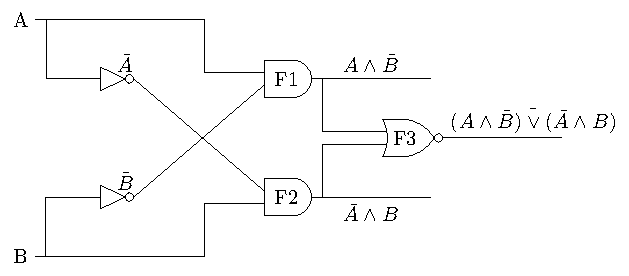
\includegraphics[width=0.8\textwidth]{reduced_circuit.pdf}
		\end{center}
	\end{answer}
	\begin{answer}
	\begin{center}
		\rowcolors{2}{gray!80!gray!50}{gray!70!gray!40}
		\begin{tabular}{|c|c|c|c|c|c|c|c|c|}
			\hline
			A & B & $\bar{A}$ & $\bar{B}$ & $F_1$ & $F_2$ & $\bar{A}\land\bar{B}$ & $A\land B$ & $F_3$ \\
			\hline
			0 & 0 & 1 & 1 &  0 & 0 & 1 & 0 & 1 \\ 
			0 & 1 & 1 & 0 & 1 & 0 & 0 & 0 & 0 \\
			1 & 0 & 0 & 1 & 0 & 1 & 0 & 0 & 0 \\
			1 & 1 & 0 & 0 & 0 & 0 & 0 & 1 & 1 \\
			 \hline
		\end{tabular}
	\end{center}
		As we see, the end result of $F_3$ has a high output when both A and B are equal, which was our intention.

	\end{answer}
\end{document}